\subsection{Desenvolver \textit{Middleware}}

O \textit{Middleware} intermediário denominado Integrador será responsável em receber as solicitações realizadas pela URA do Asterisk, após analisar deverá efetuar requisições ao \textit{WebService} do sistema GSAN, que deverá retornar as informações esperadas, até então devolver as informações essenciais ao Asterisk.
No cenário da integração proposta o sistema Integrador, deverá ser capaz de comunicar-se com o sistema Asterisk via protocolo AGI, para tanto foi utilizado um projeto \textit{Open Source} chamada Asterisk-Java, que fornece bibliotecas para comunicação com o Asterisk utilizando os protocolos comuns ao sistema, no entanto será preciso mapear as chamadas que serão realizadas.
Para cada novo serviço a ser disponibilizado, será necessário declarar uma chave de texto que será utilizada no Asterisk, representando o objeto a ser invocado, adicionados em um novo arquivo chamado \textit{fastagi-mapping.properties} da seguinte maneira, conforme a figura 13 abaixo:

\begin{figure}[!htb]
	\centering
	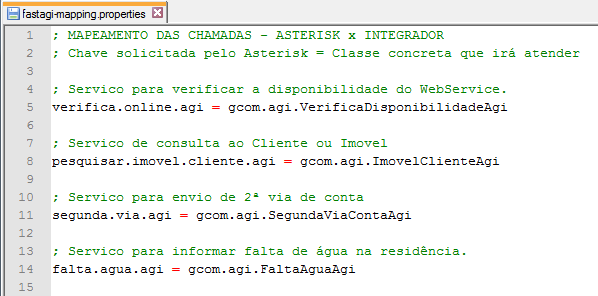
\includegraphics{figuras/mapeamento_servicos_agi.png}
	\caption{Mapeamento dos serviços para consumo via Agi}	
	Fonte - Autoria Própria
\end{figure}


Feito isso o integrador já possuirá condições de recepcionar as solicitações originadas pelo \textit{software} Asterisk utilizando o protocolo de comunicação AGI, e direcionar a chamada internamente para uma classe concreta que implemente o protocolo de comunicação utilizado, assim como a lógica de consumo aos novos serviços disponibilizados pelo \textit{WebService} do sistema GSAN.

Para cada classe concreta a ser disponibilizada será necessário estender a classe \textit{BaseAgiScript} disponibilizada pelo \textit{framework} Asterisk-Java, após estender o comportamento será necessário implementar o método service obtido pela herança da \textit{BaseAgiScript}, tal método será invocado quando a requisição for direcionada ao serviço mapeado, segue abaixo um exemplo de implementação utilizado, conforme algoritmo 1 abaixo:


\textbf{Algoritmo 1} - Novo serviço de identificação do cliente (Middleware).\\
\textbf{Entrada}: O primeiro parâmetro disponibiliza detalhes sobre a atual requisição, já o segundo contém informações e recursos para manipular o canal. (requisição, canal)
\begin{enumerate}
	\item $atenderLigação() \hspace{20 mm} \triangleright recepciona a ligação$
	\item $digitoInformado  \longleftarrow canal [cliente] \hspace{20 mm}	\triangleright	obtém dígitos informados pelo originador$
	\item \textbf{se} $valorInformado == nulo$ \textbf{então}		 
	\item  \hspace{7 mm} $tocarAudio(informar\_valor)	\hspace{20 mm}	\triangleright tocar áudio de aviso$
	\item  \hspace{7 mm} $canal [situacao] \longleftarrow erro	\hspace{20 mm}	\triangleright 	sinaliza para o canal que houve erro$
	\item \textbf{senão}
	\item  \hspace{7 mm} $ws \longleftarrow obterWebService()	\hspace{20 mm}	\triangleright	obtém uma instância do webservice cliente$
	\item  \hspace{7 mm} $retorno \longleftarrow ws.pesquisarImovelOuCliente(valorInformado) 	\hspace{20 mm}	\triangleright faz a requisição para o novo serviço do sistema GSAN$
	\item  \hspace{7 mm} $tratarRetorno(retorno) \hspace{20 mm}	\triangleright	 faz o tratamento do retorno obtido$
	\item \textbf{fim}
\end{enumerate}

Visando facilitar o consumo dos novos serviços, será gerado o \textit{WebService} cliente a partir do WSDL (\textit{Web Services Description Language}) da interface do serviço disponibilizada no sistema GSAN, utilizando o software chamado WSIMPORT disponibilizado pela \textit{Sun Microsystems}, conforme visto na figura 15:

\begin{figure}[!htb]
	\centering
	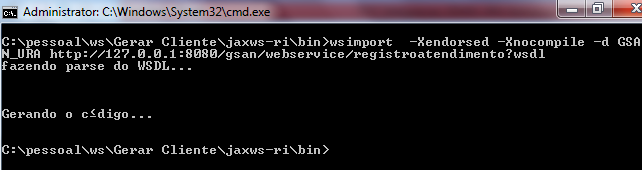
\includegraphics{figuras/gerar_wscliente.png}
	\caption{Geração do código fonte para consumo do WebService.}	
	Fonte - Autoria Própria
\end{figure}

Descrição dos parâmetros utilizados:

\begin{description}
	\item \textbf{\textit{–Xendorsed}}: Necessário para realizar a substituição dos padrões endossados do sistema, ou seja, utiliza a versão correta da JDK para realizar o parser.
	\item \textbf{\textit{–Xnocompile}}: Utilizado para gerar o código fonte não compilado, ou seja, o arquivo na extensão .java.
	\item \textbf{\textit{-d}}: Informado para determinar o diretório para onde os arquivos devem ser gerados, no exemplo o diretório se chama "GSAN\_URA".
	\item Por último a URL que disponibiliza o WSDL dos serviços. 
\end{description}



Com isso será gerado o código fonte de consumo dos serviços atualmente declarados na interface do \textit{EndPoint}, para cada modificação na interface será necessário realizar o procedimento novamente. O sistema Integrador deve ser disponibilizado em um terminal, que seja visível ao Asterisk, para que o mesmo consiga realizar requisições aos objetos mapeados anteriormente, neste trabalho o Integrador será executado no mesmo hospedeiro do Asterisk, conforme visto na figura 16 abaixo:

\begin{figure}[!htb]
	\centering
	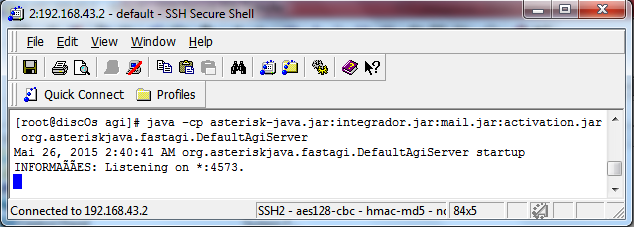
\includegraphics{figuras/executar_integrador.png}
	\caption{Executando o sistema Integrador.}	
	Fonte - Autoria Própria
\end{figure}


A instrução realizada acima executa a classe principal do \textit{framework} Asterisk-Java a \textit{ org.asteriskjava.fastagi.DefaultAgiServer}, inicializando o serviço de comunicação via AGI, sob a JVM (\textit{Java Virtual Machine}) da plataforma Java, passando como \textit{classpath} as seguintes bibliotecas: 
%Citar classpath - pendente

\begin{itemize}
	\item \textbf{\textit{asterisk-java.jar}}: biblioteca do framework utilizado para se comunicar com o Asterisk.
	\item \textbf{\textit{integrador.jar}}: o sistema integrador que integra as aplicações.
	\item \textbf{\textit{mail.jar}} e \textbf{\textit{activation.jar}}: ambos necessários no envio de email, para os casos de 2ª via de conta.	
\end{itemize}

Após estes passos o sistema Integrador já estará apto a receber solicitações do Asterisk e realizar requisições para o Sistema GSAN.